\chapter{Applicazione dei Grafi Multilivello ai Sogni} \label{cap:applicazione-dei-grafi-multilivello-ai-sogni}

Come testimoniato dalle loro svariate applicazioni, nella loro generalità e semplicità, i grafi si sono da sempre
dimostrati strutture in grado di catturare l'essenza di tanti aspetti della realtà dalla più variegata natura.
Che siano reti sociali, reti di trasporto, reti di comunicazione, reti biologiche, reti semantiche o reti di calcolo,
essi permettono di fornire un utile modello per la rappresentazione di dati complessi.
Il fatto che i grafi multi-livello siano proprio basati su grafi conferisce loro una notevole versatilità che permette
di applicarli ad una vasta gamma di problemi, tra cui l'analisi di testi in linguaggio naturale,
ed in particolare, a racconti di sogni.
Tuttavia il potenziale dei grafi multi-livello, che si basa sulla loro capacità di catturare aspetti della struttura
di un grafo ad un livello di astrazione superiore, è ciò che li rende particolarmente interessanti e che può
fornire un valore aggiunto all'analisi delle relazioni di elementi discreti, come le parole di un testo. \newline

Si noti, infatti, che nel contesto generale dell'analisi di grafi, la contrazione realizzata attraverso
l'uso di grafi multi-livello potrebbe essere utile per:
\begin{itemize}
    \item Ridurre la complessit\`a dell'analisi strutturale di un grafo, sia che esso debba essere processato
    attraverso algoritmi costosi, sia che esso debba essere graficamente visualizzato, rendendolo pi\`u facilmente
    interpretabile ed evidenziandone le caratteristiche strutturali di interesse.
    \item Studiare l'interrelazione di caratteristiche strutturali di un grafo, che rappresenti la navigabilit\`a
    di uno spazio basato su componenti fortemente connesse, cicli, cricche ecc.
    Si noti che gli spazi generati da livelli superiori al primo non potrebbero essere altrimenti ottenuti se
    non attraverso un approccio multi-livello.
    \item Stabilire il grado di connettivit\`a di un grafo, individuando la rilevanza (intesa come il numero di
    insiemi componente che rappresentano i supernodi), il numero e la dimensione delle sue contrazioni.
    \item Misurare il grado di complessit\`a dello spazio rappresentativo del grafo, in base al numero
    di nodi e archi presenti nelle contrazioni: grafi derivanti da specifici domini tendono ad avere un certo
    grado di complessit\`a legato ad un concetto spaziale, come successivamente mostrato nell'
    esempio~\ref{fig:les-miserables-graph}.
    \item Valutare l'influenza di singoli nodi e archi appartenenti al grafo di base sui livelli superiori
    del grafo multi-livello, eseguendo analisi della sensitivit\`a e della robustezza.
    Sebbene non siano presentate in questa tesi, è possibile definire delle procedure che permettano di aggiornare
    coerentemente la struttura memorizzata di un grafo multi-livello all'aggiunta e rimozione di singoli nodi e
    archi al livello base.
\end{itemize}

Nel contesto dell'analisi di testi, in particolare di racconti di sogni, con l'eventuale ausilio di strumenti di
elaborazione del linguaggio naturale, la contrazione realizzata attraverso l'uso di grafi multi-livello potrebbe
essere utile per:
\begin{itemize}
    \item Individuare contesti sintattici e possibilmente semantici di parole nel contesto del mondo onirico
    di un particolare sognatore, evidenziando l'interrelazione e la distanza tra gruppi di parole e frasi.
    \item Valutare la somiglianza sintattica di singoli racconti, individuando le macro-caratteristiche
    strutturali comuni tra i sogni di singoli individui e usarle per differenziare e catalogare più sognatori.
    \item Individuare pattern ricorrenti di parole e insiemi di parole su un corpus ampio di testi, con
    eventuale ausilio di strumenti statistici
    \item Stabilire la natura della connettività del grafo delle parole in base al numero di insiemi componente
    (gruppi di parole) e di nodi presenti nelle contrazioni.
    \item Permettere un confronto automatico dei pattern strutturali con grafi multi-livello che rappresentino
    un controllo, con l'eventuale ausilio di algoritmi che valutano il grado di somiglianza di grafi.
\end{itemize}

In questo capitolo verranno, quindi, esplorate le possibili modalità di applicazione dei grafi multi-livello allo scopo
di analisi di racconti di sogni, portando dei casi di studio reali, con l'obiettivo di evidenziarne le capacità
nell'ambito di un'analisi sintattica e semantica.
Tutti i sogni utilizzati nelle analisi sono stati prelevati da DreamBank.net \footnote{DreamBank, \url{https://dreambank.net/}}
un dataset di sogni provenienti da diverse fonti e studi di ricerca, disponibile liberamente online, mentre le
immagini dei grafi multi-livello sono state realizzate attraverso il software open-source Gephi \footnote{Gephi, \url{https://gephi.org/}}
abbinato all'uso del plugin MultiViz~\cite{s2022multivizgephipluginscalable} per la visualizzazione a più livelli.

\newpage
\section{Analisi delle differenze sintattiche tra sognatori} \label{sec:analisi-delle-differenze-sintattiche-tra-sognatori}

Come anticipato nel Capitolo~\ref{cap:mondo-dei-sogni}, nel contesto psichiatrico la rappresentazione di testi sui
sogni attraverso grafi si \`e rivelato un utile strumento a supporto della diagnosi di disturbi come la schizofrenia
o il disturbo bipolare~\cite{mota2014graph}, nonch\'e la possibilit\'a di predire l'insorgenza di patologie in
anticipo rispetto alla diagnosi clinica~\cite{mota2017thought}.
Tali studi evidenziando di come l'attenzione ad aspetti sintattici della descrizione di sogni possano fornire
informazioni significative sullo stato mentale di un individuo. Costruendo grafi in cui i nodi corrispondono a parole
e gli archi ad un loro utilizzo consecutivo, si è rivelato utile valutare aspetti come la presenza di cicli di parole
ricorrenti, la connettivit\'a delle parole e la loro organizzazione in componenti fortemente connesse.

In questa sezione verrà illustrata una possibile metodologia di analisi sintattica dei testi di singoli sogni mediante
grafi multi-livello, applicandola ai sogni di un campione di tre sognatori: Arlie, Emma e Norman.
In particolare, si cercherà di potenziare la modalità di studio proposta dalle ricerche citate, tentando di estenderla
grazie alla visione globale fornita dal grafo multi-livello e alla focalizzazione sugli aspetti che caratterizzano
l'evoluzione dei grafi delle parole nel corso delle contrazioni.

\subsection{Fase di pre-elaborazione}\label{subec:pre-elaborazione-con-NLP}
Prima di applicare la vera e propria analisi attraverso l'impiego dei grafi multi-livello al dataset di sogni, si è
ritenuto necessario effettuare una pre-elaborazione dei testi attraverso gli strumenti tipici dell'elaborazione del
linguaggio naturale.
L'NLP (in inglese \textit{Natural Language Processing}) è di fatti quella disciplina a metà tra intelligenza artificiale
e linguistica che si occupa di individuare i metodi di elaborazione e analisi di dati che si presentano sotto forma di
linguaggio naturale, ovvero di linguaggi usati dell'essere umano. \newline

La pre-elaborazione ha quindi previsto l'applicazione della seguente sequenza di fasi al corpus di sogni originario:
\begin{enumerate}
    \item \textbf{Pulizia del testo} \newline \noindent
          Questa fase ha incluso la rimozione degli spazi bianchi superflui, la standardizzazione della
          formattazione del testo e la correzione di errori ortografici o di incoerenze. È stata inoltre eseguita la
          rimozione della punteggiatura, snellendo ulteriormente i dati testuali. Tali procedure di pulizia sono
          essenziali per garantire la qualità e la coerenza dei dati in ingresso, migliorando così l'affidabilità
          dell'analisi.
    \item \textbf{Tokenizzazione} \newline \noindent
          Questa fase ha comportato la suddivisione del testo in parole singole dette \textit{token},
          passaggio fondamentale nell'elaborazione del linguaggio naturale, creando la base per le fasi successive.
    \item \textbf{Rimozione delle stop words} \newline \noindent
          Le \textit{stop words} sono parole comuni (come ``the'', ``is'', ``at'', ``which'' e ``on'') che tipicamente
          non hanno un ruolo significativo nei compiti di NLP, specialmente in quelli legati ad analisi semantiche.
          In questo caso, la loro rimozione può certamente aiutare a concentrare l'analisi sulle parole più ricche di
          contenuto nelle narrazioni dei sogni, riducendo significativamente il rumore nei dati e mettendo in evidenza
          i termini più salienti.
    \item \textbf{Lemmatizzazione} \newline \noindent
          La lemmatizzazione è un processo che riduce le parole alla loro forma base, chiamata \textit{lemma}.
          Ad esempio, ``running'' verrebbe lemmatizzato in ``run'' e ``better'' in ``good''.
          Questo passaggio aiuta a ridurre le diverse declinazioni delle parole ai loro concetti di base, riducendo
          la dimensionalità dei dati testuali e rivelando, potenzialmente, schemi sottostanti in modo più chiaro.
    \item \textbf{Costruzione del grafo delle parole} \newline \noindent
          Infine, è stato costruito un grafo diretto basato sulle singole parole all'interno delle sequenze
          di lemmi associate a ogni sogno. Tali parole, in quanto prese singolarmente rispetto alla sequenza
          di appartenenza, si definiscono \textit{unigrammi}. In questo grafo, quindi, ogni nodo rappresenta
          un unigramma univoco, con una proprietà ``peso'' che indica il numero di occorrenze di quell'unigramma
          nell'intero corpus di sogni.
          Gli archi orientati del grafo collegano gli unigrammi dei lemmi che appaiono seguitamente nella
          sequenza associata ad ogni sogno.
          Per questo motivo, ad ogni arco corrisponde un \textit{bigramma}, ovvero un accostamento ordinato di due parole.
          Il peso di ciascun arco rappresenta il numero di occorrenze di quello specifico accostamento ordinato nel testo.
          In questo modo, la struttura del grafo cattura non solo le relazioni sequenziali tra le parole nei sogni,
          ma anche la frequenza e la forza di queste parole e relazioni.
\end{enumerate}

\begin{figure}[h!]
    \centering
    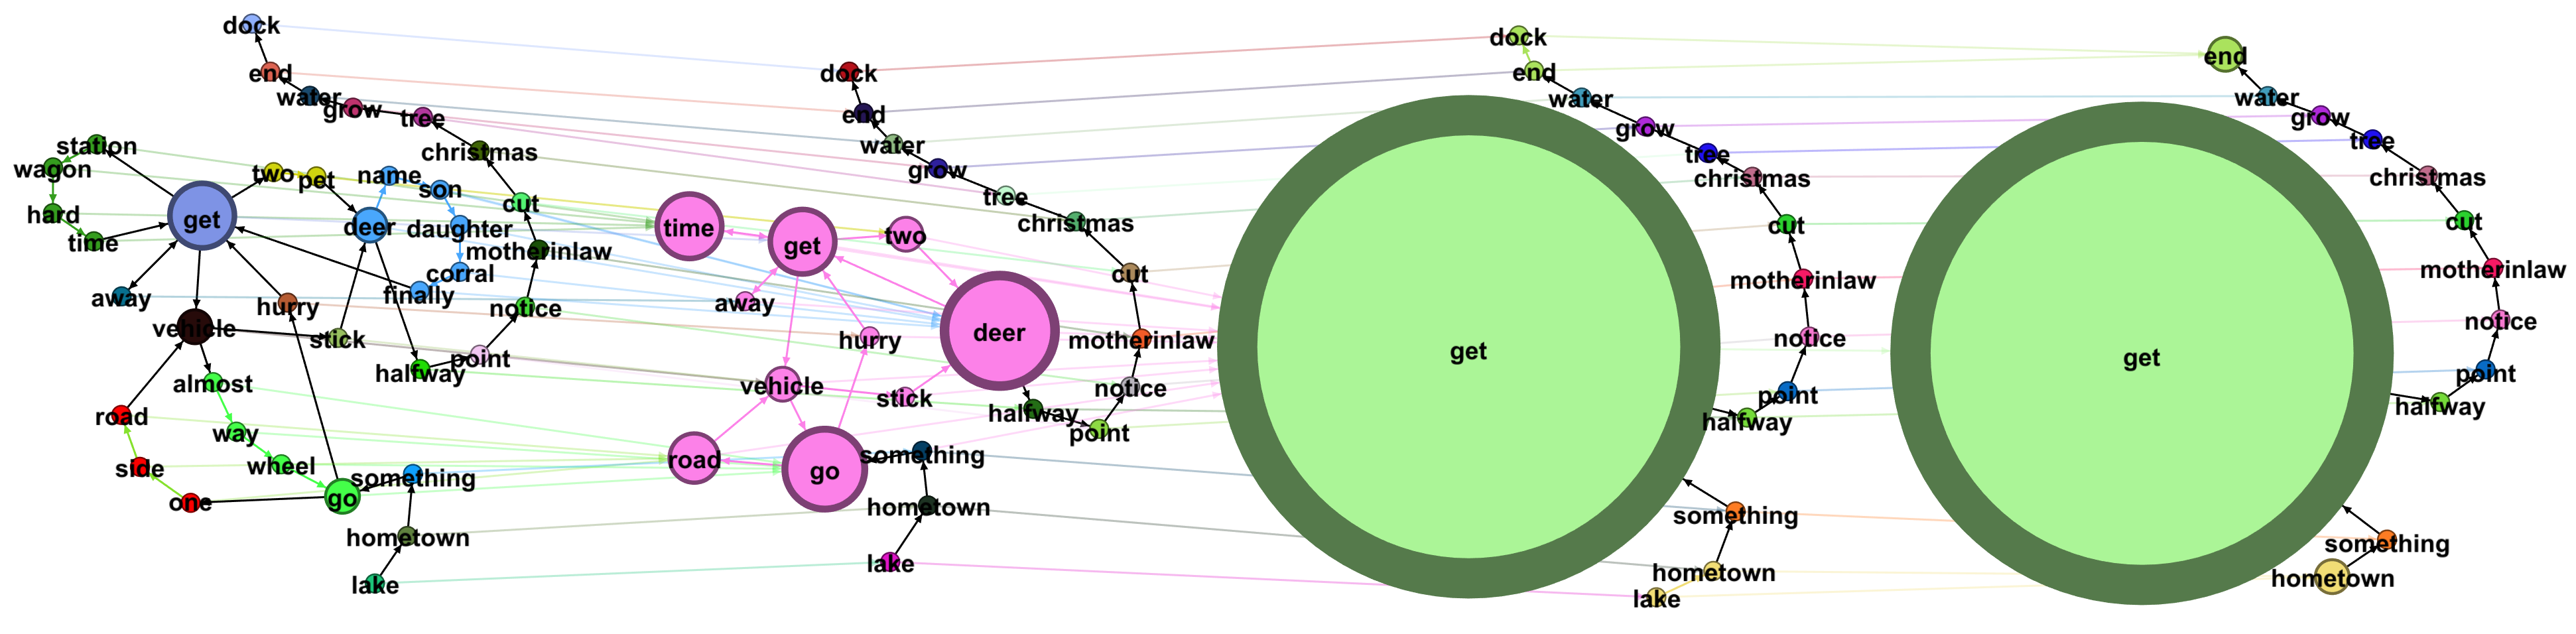
\includegraphics[width=1\textwidth]{Immagini/arlie_dream_graph_example}
    \caption{Grafo multi-livello di un sogno di Arlie}
    \label{fig:arlie-dream-graph}
\end{figure}

Utilizzando il grafo delle parole $G$ così prodotto come input per la costruzione di grafo multi-livello
$M = (G, \Gamma)$, è quindi stato possibile rappresentare i sogni di Emma, Arlie e Norman in un'unica struttura,
dove i supernodi rappresentano parole, concetti e pensieri a diversi livelli di astrazione, mentre i super-archi
rappresentano le relazioni tra tali elementi quando sono correlati.
In Figura~\ref{fig:arlie-dream-graph} è mostrato un esempio di grafo delle parole costruito a partire da un sogno di Arlie, e dei
relativi livelli di astrazione ottenuti attraverso la contrazione del grafo.
In particolare, l'esempio mostra il grafo multi-livello risultante dall'applicazione di schemi di contrazione per
circuiti semplici, componenti fortemente connesse e stelle.
La funzione di contrazione per stelle rappresenta un ulteriore livello di astrazione in cui tutti i nodi su cui è
incidente un unico arco che li collega ad un nodo centrale vengono contratti in un unico supernodo.
Nel caso delle parole, il centro di una stella può rappresentante il concetto di base comune a tutti i nodi contratti,
in quanto loro unico punto di collegamento con le altre parole del grafo.

I grafi multi-livello così prodotti sono stati quindi utilizzati come base per l'analisi multi-livello dei sogni,
come descritto nella sezione successiva.

\subsection{Analisi dei risultati}
A partire dall'analisi di un dataset di narrazioni di sogni provenienti da sedici individui si è seguita la
metodologia precedentemente descritta, raccogliendo dati statistici sulle caratteristiche topologiche
dei grafi a vari livelli delle gerarchie prodotte per ciascun sognatore.
In questa parte l'attenzione verrà rivolta a tre particolari sognatori dei sedici originali: Arlie, Emma e Norman.
Arlie è stata identificata come un sognatrice con grafi delle parole aventi parametri strutturali che più si
avvicinano alle medie del campione, mentre Emma e Norman sono stati scelti per alcune caratteristiche atipiche
che li differenziano dal resto del gruppo.

Il grafo multi-livello $M = (G, \Gamma)$ scelto per l'elaborazione del grafo delle parole $G$ prodotto a partire
da ciascun sogno prevede una sequenza di sette funzioni di contrazione che sono, rispettivamente:
\begin{itemize}
    \item \eqmakebox[things][l]{$f_{C_1}$}
    $ \begin{aligned}[t]
      \text{funzione di contrazione per circuiti semplici.}
      \end{aligned} $
    \item \eqmakebox[things][l]{$f_{C_2}$}
    $ \begin{aligned}[t]
      \text{funzione di contrazione per componenti fortemente connesse.}
      \end{aligned} $
    \item \eqmakebox[things][l]{$f_{C_3},\ldots,f_{C_7}$}
    $ \begin{aligned}[t]
      \text{funzioni di contrazione per stelle.}
      \end{aligned} $
\end{itemize}

Ciascuno dei grafici presentati a seguire comprende tre traiettorie distinte, ognuna corrispondente ai dati
dei tre sognatori selezionati, ottenuti da un insieme di 221, 1252 e 669 narrazioni, rispettivamente.
Per ciascun insieme di narrazioni legate ai particolari sognatori, si sono selezionati i sogni con un numero di
occorrenze di lemmi compreso tra 15 e 300 per narrazione, approssimativamente corrispondenti a sogni
di lunghezze che variano dalle 30 alle 750 parole.
I grafici mostrano l'evoluzione di una certa proprietà dei grafi a ciascun livello della gerarchia,
dove il livello $0$ rappresenta la struttura originale del grafo.
L'asse delle ordinate quantifica la proprietà, mentre l'asse delle ascisse delinea i livelli del grafo multi-livello.

A causa della significativa variazione nel numero medio di lemmi tra le narrazioni dei sognatori — per precisione
48,47 per Arlie, 38,57 per Emma e 28,80 per Norman — i dati sensibili alla lunghezza del sogno sono stati normalizzati a un
valore percentuale relativo al conteggio dei lemmi del sogno originale.
A partire da osservazioni effettuate sul dataset, infatti, dati come il numero di nodi e archi, il peso dei nodi,
la dimensione degli insiemi componente e il numero (ma non la lunghezza) delle basi cicliche risultano essere tutti
linearmente influenzati dal numero di lemmi considerati in ciascun sogno.

\newpage

\begin{wrapfigure}{R}{0.5\textwidth}
    \vspace{-5pt}
    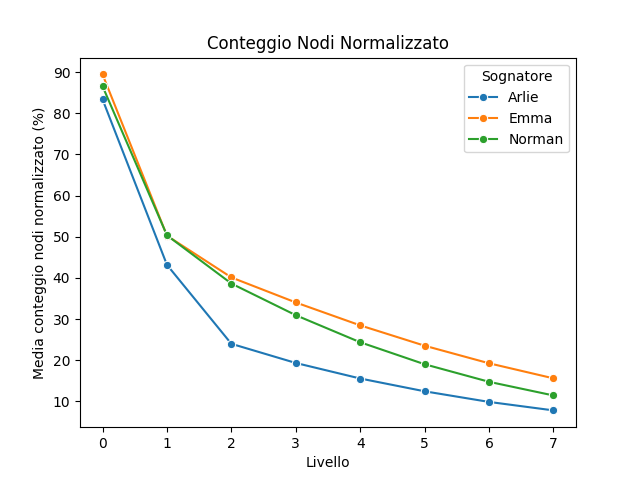
\includegraphics[width=0.55\textwidth]{Immagini/conteggio_nodi_normalizzato}
    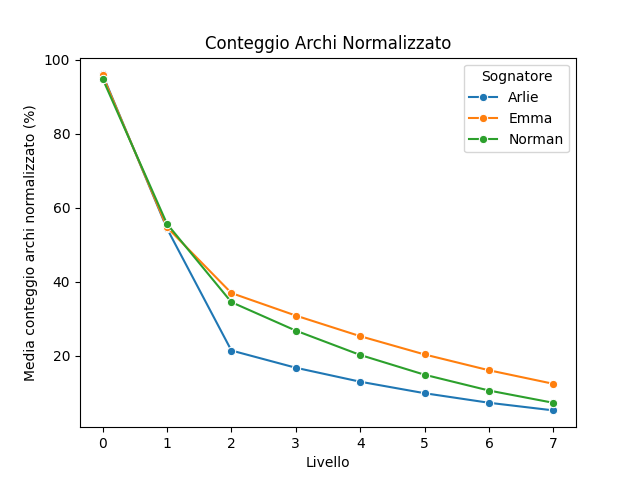
\includegraphics[width=0.55\textwidth]{Immagini/conteggio_archi_normalizzato}
    \caption{Statistiche sulle dimensioni dei grafi}\label{fig:node_edge_count}
    \vspace{-5pt}
\end{wrapfigure}

Nella Figura~\ref{fig:node_edge_count}, in alto, è mostrato il grafico del conteggio dei nodi, il quale illustra
l'evoluzione della quantità di nodi nei vari livelli.
I cali significativi delle traiettorie che scendono velocemente a partire da un valore alto indicano una struttura
di nodi inizialmente complessa che subisce una rapida semplificazione.
I dati di Arlie mostrano una discesa più ripida, suggerendo una veloce contrazione della struttura iniziale sin
dai primi schemi di contrazione.
I dati di Norman ed Emma presentano un tasso di declino più contenuto, mantenendo una riduzione coerente rispetto
allo specifico schema di contrazione, indicativo di strutture meno organizzate.

Il grafico del conteggio degli archi imita l'analisi ottenuta dal conteggio dei nodi, fornendo un'idea più chiara
della complessità delle strutture.
Analogamente al conteggio dei nodi, un valore iniziale alto sulle ordinate seguito da un brusco calo suggerisce
una connettività iniziale densa che subisce una significativa semplificazione.
I dati sui sogni di Arlie mostrano una densità di archi ordinaria con un marcato declino al livello $2$, indicando una
sostanziale interconnessione di parole.
Essendo che tali interconnessioni derivano da una quantità di archi al livello $1$ proporzionalmente
paragonabile a quella degli altri due sognatori, questo aspetto potrebbe suggerire una maggiore qualità delle relazioni
tra le parole nei sogni di Arlie, intesa come una più equa distribuzione degli archi tra parole e cicli di parole.

\begin{wrapfigure}{L}{0.5\textwidth}
   \vspace{-5pt}
    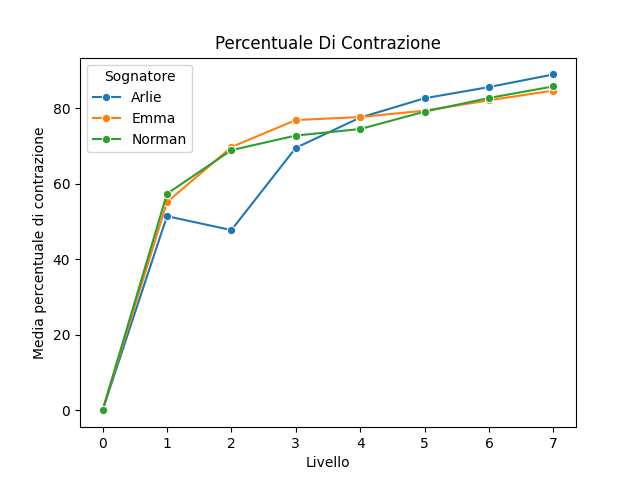
\includegraphics[width=0.55\textwidth]{Immagini/percentuale_di_contrazione}
    \caption{Statistiche sulla contrazione}\label{fig:contraction_percentage}
   \vspace{-5pt}
\end{wrapfigure}

Il grafico in Figura~\ref{fig:contraction_percentage} permette di arricchire la visione fornita dai grafici precedenti,
mostrando la percentuale di contrazione dei nodi di ciascun livello, calcolata considerando la quantità di nodi del
livello rispetto a quella del livello precedente.
Le linee indicano che, mentre Emma e Norman presentano solo lievi differenze nelle prime contrazioni per stelle, i dati
di Arlie mostrano una divergenza più significativa nel processo di contrazione delle componenti fortemente connesse.
Questa informazione, combinata con le quelle fornite dai grafici precedenti, suggerisce che molti nodi vengono esclusi
dalle aggregazioni principali, portando a una struttura più frammentata.
Tuttavia, questa struttura si semplifica rapidamente nei livelli successivi, indicando che la maggior parte dei nodi
orbita nelle immediate vicinanze di massicce aggregazioni principali.

\begin{wrapfigure}{R}{0.5\textwidth}
    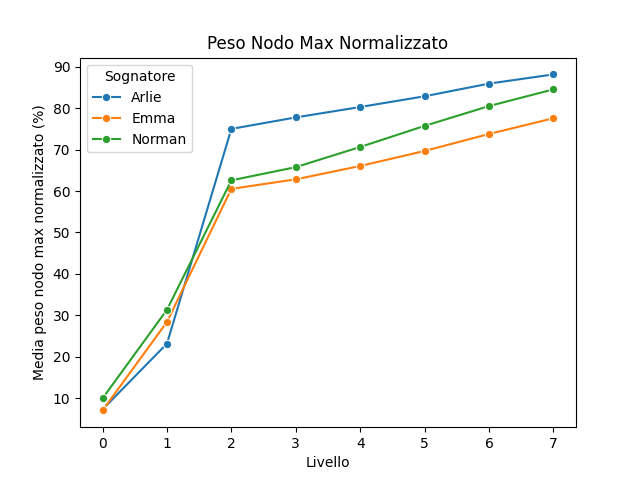
\includegraphics[width=0.55\textwidth]{Immagini/peso_nodo_max_normalizzato}
    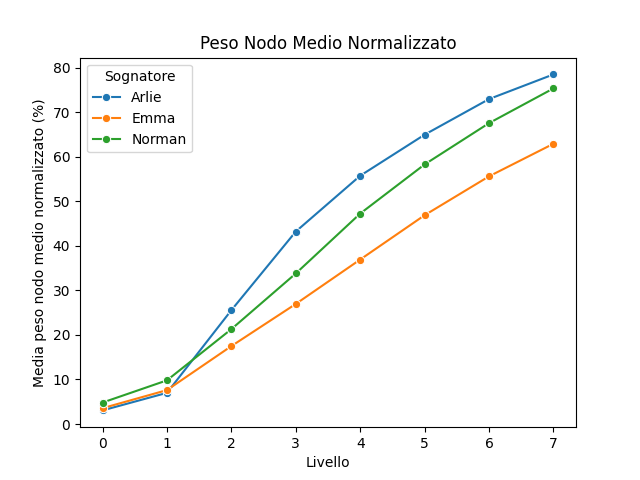
\includegraphics[width=0.55\textwidth]{Immagini/peso_nodo_medio_normalizzato}
    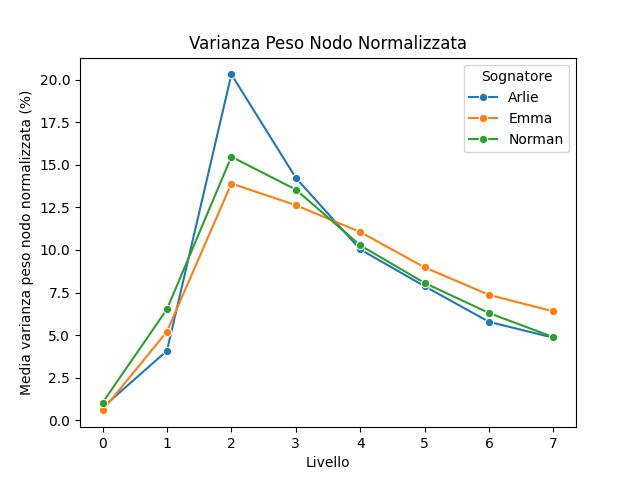
\includegraphics[width=0.55\textwidth]{Immagini/varianza_peso_nodo_normalizzata}
    \caption{Statistiche sui pesi dei nodi}\label{fig:node_weight}
\end{wrapfigure}

In Figura~\ref{fig:node_weight} i grafici danno un'idea dell'evoluzione della distribuzione del peso dei nodi.
Al livello iniziale, i dati di Arlie mostrano un peso medio dei nodi moderato, seguito da un marcato aumento nel
corso dei livelli superiori.
Questo modello suggerisce che, mentre le strutture iniziali possiedono nodi di moderata importanza,
l'aggregazione per componenti fortemente connesse amplifica particolarmente la loro rilevanza, risultando in
aggregazioni altamente pesanti.
Ciò non risulta particolarmente evidente nel caso degli altri due sognatori che mantengono un incremento del peso
medio più tendente al rettilineo.
In particolare, i dati di Emma dimostrano un aumento moderato ma costante del peso medio dei nodi, indicativo di
una struttura iniziale equilibrata in cui i nodi acquisiscono gradualmente importanza attraverso i livelli successivi.
D'altra parte, i dati di Norman mostrano un aumento leggermente più pronunciato, a partire dai cicli fino ai
livelli superiori, riflettendo una più bassa dispersione delle singole parole rispetto a Emma, e una maggiore
inclinazione all'aggregazione, specialmente per le formazioni a stella.
Il grafico della varianza sul peso dei nodi fornisce informazioni sull'equilibrio interno delle strutture rispetto
alla loro importanza.
I dati di Arlie mostrano un forte aumento della varianza, con un picco notevole al livello $2$, indicando una convergenza
di molti nodi verso poche aggregazioni altamente significative ed evidenziando nuovamente l'importanza delle componenti
fortemente connesse nel processo di aggregazione.
I dati di Emma presentano una varianza più alta ai livelli superiori, suggerendo la frequente presenza di nodi
poco pesanti che rimangono distaccati dalle aggregazioni principali e che, quindi, sono generalmente distanti, poco
connessi o situati in fondo a cammini che rappresentano vicoli ciechi.

\newpage

\begin{wrapfigure}{L}{0.5\textwidth}
    \vspace{-10pt}
    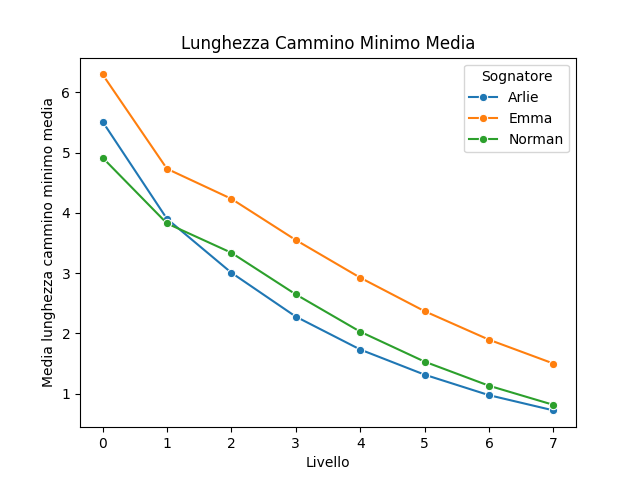
\includegraphics[width=0.55\textwidth]{Immagini/lunghezza_cammino_minimo_media}
    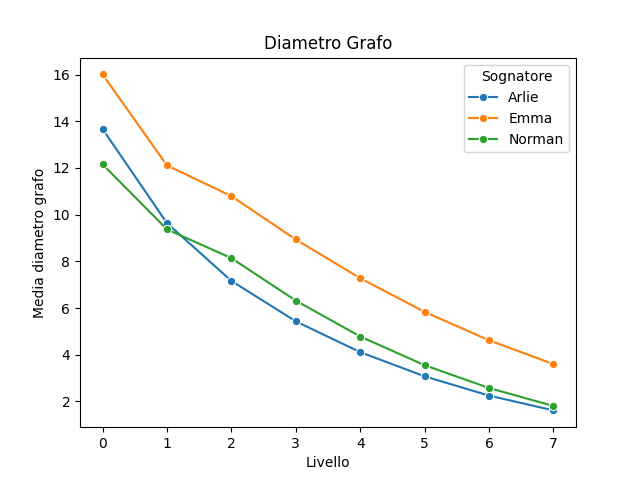
\includegraphics[width=0.55\textwidth]{Immagini/diametro_grafo}
    \caption{Statistiche sui cammini}\label{fig:paths}
    \vspace{-10pt}
\end{wrapfigure}

Il grafico delle medie dei cammini minimi in Figura~\ref{fig:paths} rappresenta l'evoluzione della lunghezza media di
tali cammini attraverso i diversi livelli dei grafi.
La misura è calcolata sulla versione non orientata di ciascun grafo come la distanza media tra ciascuna coppia di
nodi in termini di archi.
Valori iniziali più alti indicano strutture iniziali più estese, le quali normalmente riducono tale caratteristica
contraendosi attraverso i livelli successivi.
I dati di Emma iniziano con cammini mediamente lunghi, da cui si deduce la presenza percorsi inizialmente isolati
che diventano via via più compatti rispetto al resto del grafo, specialmente con la contrazione dei cicli.
Tuttavia, i grafi delle parole di Emma dimostrano di mantenere un'elevata lunghezza media, corroborando l'ipotesi
della frequente presenza di lunghi vicoli ciechi.
I dati di Norman mostrano cammini di lunghezze più moderate, imitando l'andamento di Emma,
mentre i dati di Arlie presentano cammini inizialmente più lunghi e con declino più graduale, indicando strutture di
percorso più semplici.
Il secondo grafico nella stessa figura mostra l'evoluzione del diametro del grafo, parametro strettamente legato
alla lunghezza dei cammini minimi, definito come il cammino minimo di lunghezza massima tra tutte le coppie di nodi.
Diametri iniziali più alti indicano strutture più estese.
Questo grafico segue accuratamente quello precedente, indicando che, per tutti e tre i sognatori, le forme del grafo
tra i livelli non sono deformate e contengono nodi approssimativamente equidistanti.

Il grafico del conteggio delle basi cicliche in Figura~\ref{fig:cycle_basis} quantifica la presenza di collegamenti
circolari tra parole o gruppi di parole, considerando la versione non orientata dei grafi.
Le basi cicliche rappresentano i cicli fondamentali del grafo non ulteriormente scomponibili in sotto-cicli.
Sono dette ``basi'' in quanto a partire da esse è possibile comporre tutti gli altri cicli attraverso una operazione di
unione degli archi che li compongono in or esclusivo.
I dati di Norman mostrano un alto conteggio iniziale dei cicli seguiti da un brusco calo, indicando la presenza di molti
cicli orientati tra le basi cicliche che vengono riconosciute nella prima funzione di contrazione.
I dati di Arlie presentano più basi cicliche che non sono facilmente contratte al primo livello di contrazione,
indicando una maggiore presenza di connessioni cicliche nascoste che non seguono un semplice percorso unidirezionale.
I dati di Emma mostrano meno cicli con una diminuzione costante, indicando la presenza di strutture più lineari.
Queste informazioni, combinate ai dati del grafico sulla lunghezza delle basi cicliche, suggeriscono che i sogni di
Norman contengono più cicli, anche se più piccoli, mentre i sogni di Emma contengono una minor quantità di cicli,
seppur generalmente più grandi.
Tuttavia, la distinzione sulla lunghezza tra Emma e Arlie può essere osservata solo nel grafo al livello $1$, suggerendo
che, a differenza di Arlie, le basi cicliche di Emma sono ottenute prevalentemente da insiemi di parole che si
conseguono nella narrazione originale del sogno, nonostante consistano di un alto numero di lemmi.

\begin{figure}[t]
    \hspace{-5pt}
    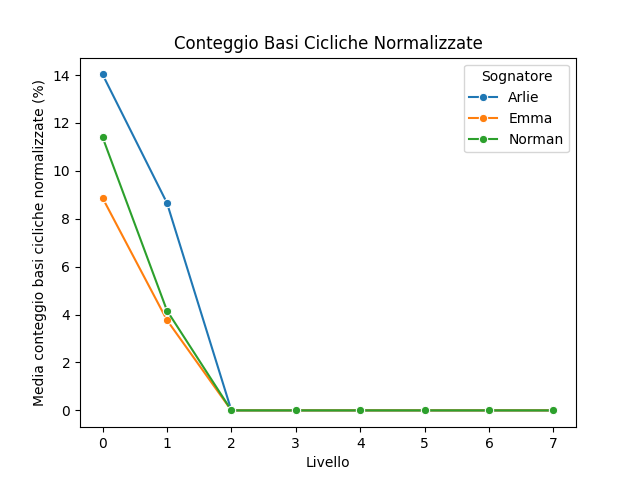
\includegraphics[width=0.55\textwidth]{Immagini/conteggio_basi_cicliche_normalizzate}
    \hspace{-20pt}
    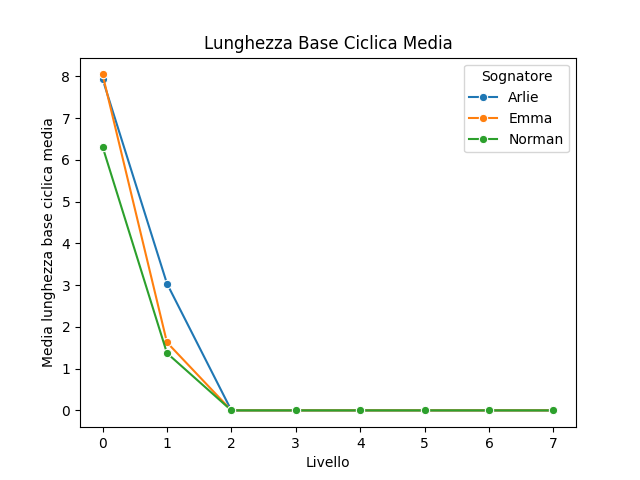
\includegraphics[width=0.55\textwidth]{Immagini/lunghezza_base_ciclica_media}
    \hspace{-5pt}
    \vspace{-10pt}
    \caption{Statistiche sulle basi cicliche}\label{fig:cycle_basis}
\end{figure}

\begin{wrapfigure}{R}{0.5\textwidth}
    \includegraphics[width=0.55\textwidth]{Immagini/densità_grafo}
    \caption{Statistiche sulla densità}\label{fig:density}
\end{wrapfigure}

La Figura~\ref{fig:density} illustra la densità media dei grafi per ciascun livello, dove la densità di un grafo è
definita come il rapporto tra il numero di archi nel grafo e il numero di archi possibili.
Tutti e tre i sognatori iniziano con basse densità iniziali del grafo che aumentano attraverso i primi livelli di
contrazione.
Oltre che essere una naturale conseguenza della riduzione della dimensione del grafo, questo indica che le strutture
iniziali di singole parole sparse diventano più interconnesse quando i nodi rappresentano aggregazioni di parole
correlate.
Le narrazioni di Arlie mostrano l'aumento di densità più elevato nel corso dei primi livelli di contrazione,
suggerendo un'interconnessione più complessa tra le componenti fortemente connesse, che si semplifica
rapidamente nei livelli successivi.
Livelli di densità bassi ai livelli superiori possono anche indicare una maggiore tendenza alla presenza di
un unico grande cluster di parole.
Osservando gli altri due sognatori, è interessante notare che, mentre i sogni di Norman mostrano una densità più alta
rispetto a quelli di Emma nei livelli iniziali, i dati dei due sognatori convergono a valori simili nei livelli
superiori, indicando un livello simile di interconnessione tra le aggregazioni principali.

\begin{figure}[t]
    \hspace{-5pt}
    \includegraphics[width=0.55\textwidth]{Immagini/coefficiente_di_assortatività_peso}
    \hspace{-20pt}
    \includegraphics[width=0.55\textwidth]{Immagini/coefficiente_di_assortatività_grado}
    \hspace{-5pt}
    \vspace{-10pt}
    \caption{Statistiche sull'assortatività}\label{fig:assortativity}
\end{figure}

Il grafico del coefficiente di assortatività dei pesi in Figura~\ref{fig:assortativity} fornisce informazioni
sull'evoluzione di tale valore tra i singoli nodi.
L'assortatività è un parametro che misura la tendenza dei nodi con determinate caratteristiche numeriche a collegarsi
con nodi aventi caratteristiche simili e, in questo caso, indica la tendenza dei nodi con pesi simili a connettersi tra
loro.
Un coefficiente positivo suggerisce la presenza di una tendenza per i temi predominanti a connettersi direttamente
tra loro, mentre un coefficiente negativo indica una tendenza per i nodi pesanti a connettersi con nodi di peso esiguo.
Questo potrebbe essere particolarmente rilevante nei livelli avanzati, dove i temi principali del sogno sono già ben
definiti.
I sogni di Norman sono soggetti ad un evidente calo dell'assortatività ai livelli alti, indicando, possibilmente,
la presenza ricorrente di una contrazione principale circondata da nodi meno importanti.
I dati di Emma, invece, mostrano una tendenza più stabile, suggerendo che le aggregazioni principali sono tipicamente
interconnesse tra loro e che non possano facilmente essere ridotte a un singolo nodo che rappresenti una formazione a
stella.

\nlparagraph{Confronto con gli studi correlati}

Studi correlati già citati, che riguardano tecniche di analisi dei sogni basate su grafi, hanno osservato differenze
nelle caratteristiche topologiche dei grafi a partire da gruppi di persone pre-classificate come sognatori sani,
schizofrenici o bipolari.
In particolare, i grafi associati ai sogni di pazienti schizofrenici sono stati valutati come grafi generalmente
piccoli e poco connessi, con basso numero di cicli, un elevato diametro rapportato alla dimensione del grafo e un
basso coefficiente di clustering, il quale indica la tendenza dei nodi a formare cluster densamente connessi.
I grafi dei pazienti bipolari, sebbene abbiano dimostrato avere un numero inferiore di caratteristiche che permettono
di distinguerli rispetto al gruppo di controllo, sono prevalentemente caratterizzati da alta connettività, alta densità
e alto coefficiente di clustering, abbinato alla maggiore presenza di cicli brevi e un basso diametro.
Tuttavia la caratteristica che ha permesso di caratterizzare e riconoscere distintamente il gruppo di controllo
dagli altri due è la presenza e la dimensione delle componenti fortemente connesse: i sognatori del controllo hanno
mostrato la dimensione maggiore tra tutti, seguiti dai bipolari e, per ultimi, gli schizofrenici. \newline

Per via del fatto che i dati ottenuti in questa analisi non sono corredati da informazioni riguardanti lo stato di
salute mentale dei sognatori, i risultati sono stati confrontati con quelli degli studi precedenti al fine
di trarre delle ipotesi su una possibile classificazione dei sognatori.
I risultati dell'analisi multi-livello si correlano alle scoperte già consolidate suggerendo che Arlie potrebbe essere
collocata nel gruppo di controllo, a causa dell'alta rilevanza delle componenti fortemente connesse nel processo di
contrazione e di altri parametri riguardanti la connettività e l'alto grado dei nodi.
Questa ipotesi è supportata dal fatto che i grafici di Arlie si conformano ai valori medi dei sedici sognatori nel
dataset.
Al contrario, Emma ha presentato caratteristiche tipiche dei pazienti schizofrenici, come un diametro del grafo
elevato e un basso coefficiente di clustering, indicando nodi poco connessi.
Dai dati di Norman, nel mentre, è emersa una rilevanza dei cicli e un alto coefficiente di clustering, che potrebbero
essere considerate qualità simili ai sogni dei pazienti bipolari.
Si noti, tuttavia, che molti altri sono stati gli aspetti emersi dall'analisi multi-livello, i quali hanno fornito una
visione più completa sui sognatori rispetto a quella che si sarebbe ottenuta da un'analisi a livello singolo.


\newpage
\section{Analisi dei contesti semantici di un sognatore}\label{sec:analisi-dei-contesti-semantici-di-un-sognatore}

L'estrapolazione di informazioni legate al significato delle parole a partire da aspetti sintattici \`e un
principio fondamentale della semantica computazionale, noto come \textit{ipotesi distribuzionale}, che si basa sul
principio per cui il significato di una parola \`e determinato dal suo contesto di utilizzo, e che le parole che
appaiono nello stesso contesto tendono ad avere significati simili.\newline
In questa sezione verrà esplorato un caso di studio, risultato del tentativo di usare il modello dei grafi multi-livello
allo scopo di individuare dei contesti di parole di valenza sintattica e semantica all'interno del mondo onirico
di una particolare sognatrice.
Daremo forma allo spazio delle parole di Emma a partire da un vasto corpus di racconti di sogni, e analizzeremo la
struttura del grafo multi-livello risultante.

\subsection{Fase di pre-elaborazione}

Per poter procedere con l'analisi dei sogni di Emma affinché si potesse costruire un grafo delle parole
da cui poter cogliere aspetti semantici, si è ritenuto necessario aggiungere dei passaggi ulteriori
al processo di pre-elaborazione descritto nella sottosezione~\ref{subec:pre-elaborazione-con-NLP}.
In particolare, si è rivelato utile allo scopo di un'analisi semantica,
un filtraggio delle parole meno frequenti rispetto all'intero corpus di sogni di Emma.
Questo passaggio è stato eseguito per ridurre la complessità del testo e concentrare l'analisi sui
termini più rilevanti e significativi, con l'obiettivo di individuare le tematiche principali trattate
nei sogni e l'ordine con cui esse appaiono nei testi.
Un'altra possibile interessante fase di pre-elaborazione ulteriore è quella dell'estrapolazione di categorie
specifiche di parole.
Attraverso tecniche di NLP come il Part-of-Speech (POS) tagging, ciascuna parola può essere etichettata con la sua
categoria grammaticale di appartenenza, come quella dei sostantivi, verbi, aggettivi, avverbi, ecc.
Con la tecnica di Named Entity Recognition (NER) tagging è possibile, invece, identificare le entità di interesse
all'interno del testo, categorizzando elementi come persone, luoghi e organizzazioni.
A partire da queste categorizzazioni, tutte le parole che non sono etichettate in una particolare
categoria vengono filtrate. Lo scopo di questa fase potrebbe essere quello di concentrare l'analisi sulle parole che
sono considerate le parti del testo più significative e ricche di contenuto, o semplicemente focalizzare l'analisi
su un aspetto di interesse.


\nlparagraph{Connettività del grafo delle parole}

Sebbene il grafo delle parole risultante dalla pre-elaborazione di tutti i sogni di un particolare sognatore
sia frutto di un processo di semplificazione e riduzione della complessità del testo, la sua analisi diretta
attraverso l'uso del grafo multi-livello ne ha rivelato sin da subito la sua elevata connettività derivante dalla
natura del linguaggio naturale: parole e concetti possono essere strettamente legati (e quindi ``vicini'') ad un
ampio numero di altri concetti che a loro volta possono collegarsi direttamente ad altri concetti sparsi per il grafo.
Il risultato è uno spazio fortemente ``aggrovigliato'' che non favorisce la formazione di gruppi di parole distinti e
ben definiti e che, di conseguenza, non favorisce un processo di contrazione di qualità nella
gerarchia del grafo multi-livello.

Per rendere chiaro questo aspetto, si prenda come esempio il grafo multi-livello $M = (G, \langle f_{C_1}, f_{C_2}\rangle)$
rappresentato in figura~\ref{fig:les-miserables-graph}, il cui grafo $G$ rappresenta il grafo delle relazioni di
co-apparizione dei personaggi del romanzo \textit{Les Misérables} di Victor Hugo,
e le cui funzioni di contrazione $f_{C_1}$ e $f_{C_2}$ rappresentano rispettivamente le funzioni di contrazione
per cricche non reciproche e stelle.
Appare evidente di come la struttura del grafo $G$ sia stata contratta con un elevato tasso di contrazione,
producendo una struttura notevolmente più semplice e facilmente interpretabile. Per via degli schemi di
contrazione scelti, appare evidente come la struttura originale del grafo abbia rivelato la sua ordinatezza ai livelli
superiori: in media i personaggi del romanzo possono apparire assieme ad una cerchia ristretta di altri personaggi,
ad eccezione di personaggi principali che risultano collegarsi a questi gruppi più o meno isolati di nodi.
Questo rispecchia in parte la natura dello spazio bidimensionale in cui i personaggi sono collocati: personaggi
appartenenti a luoghi distanti difficilmente appariranno insieme. I personaggi principali, in quanto seguiti
nella narrazione nel mentre che si spostano nello spazio, permettono di rompere questa dimensionalità, e risultano
essere collegati a nodi distanti tra loro.

\begin{figure}[h]
    \centering
    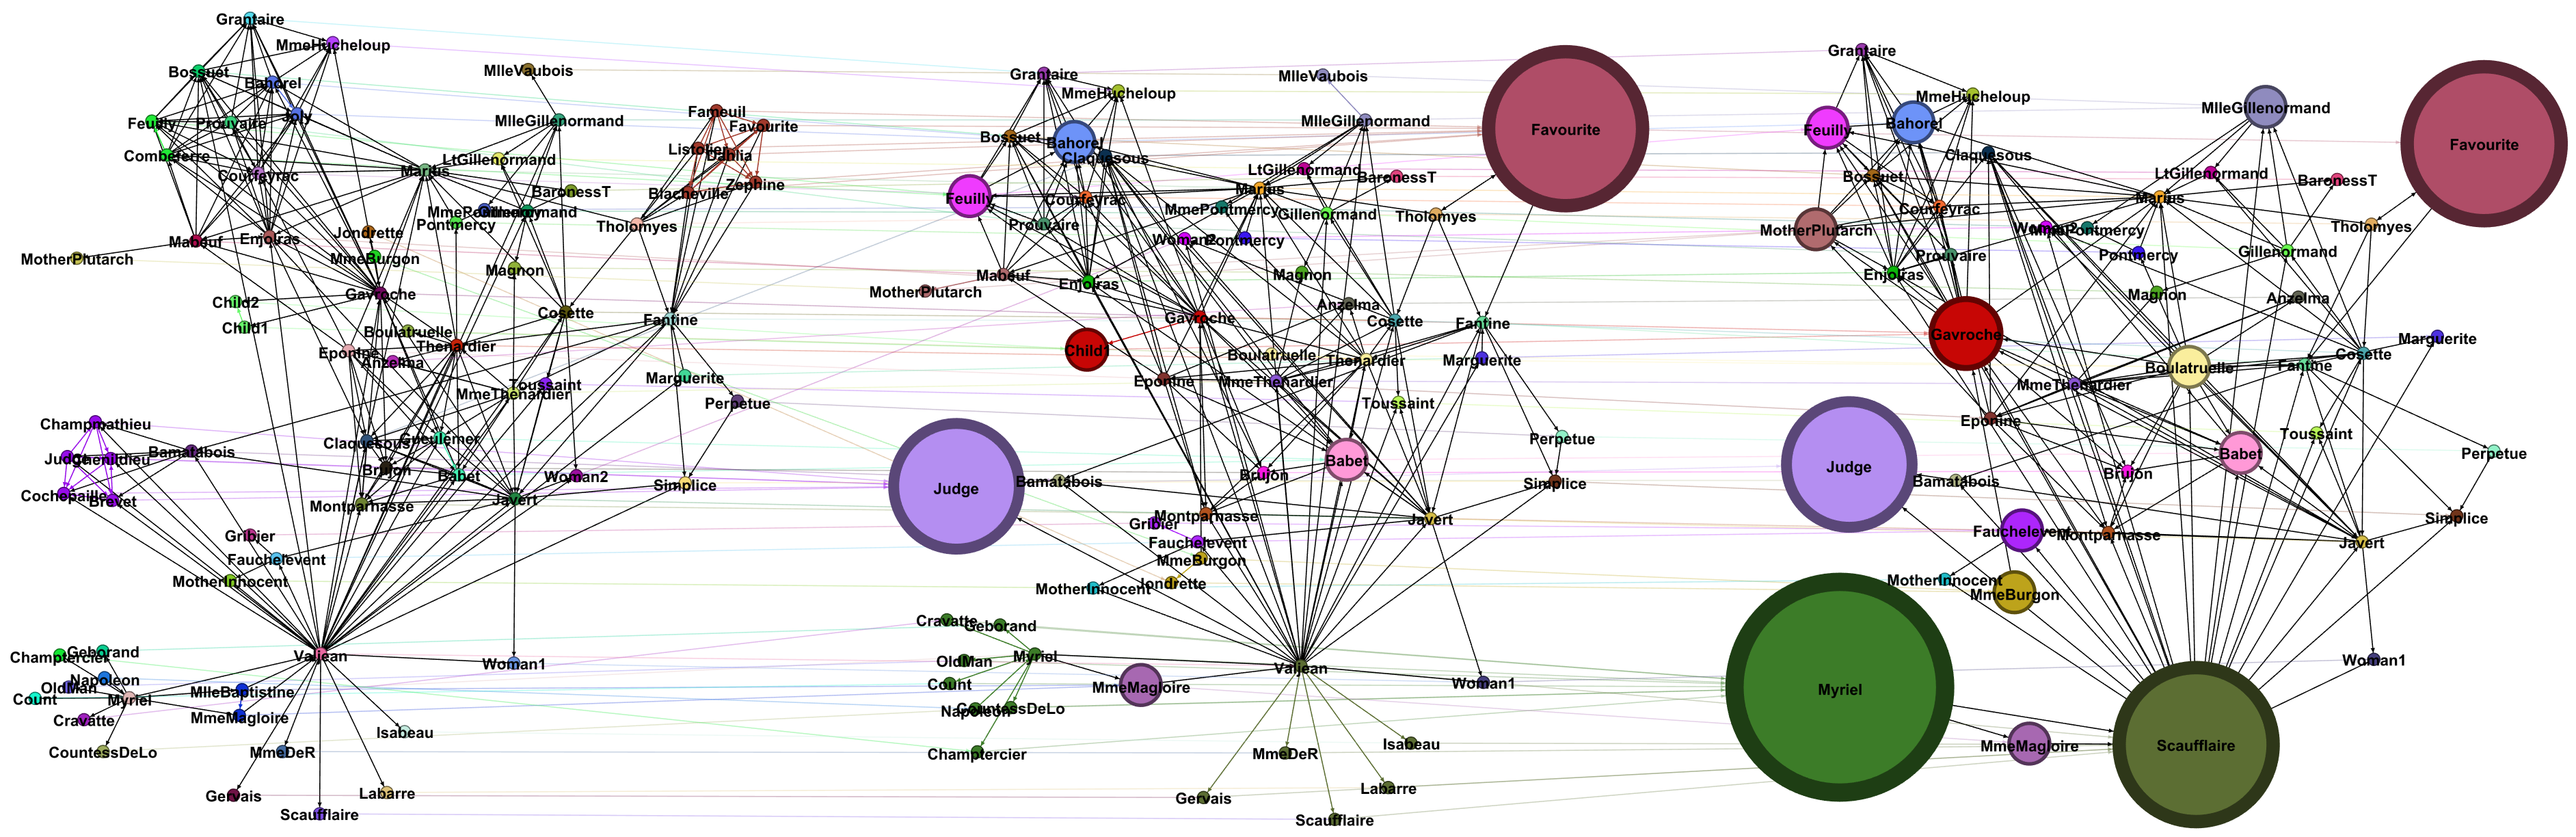
\includegraphics[width=1\textwidth]{Immagini/les_miserables_example}
    \caption{Grafo multi-livello delle co-apparizioni in \textit{Les Misérables}}
    \label{fig:les-miserables-graph}
\end{figure}

Per risolvere questo problema legato all'alta connettività del grafo delle parole, si è deciso di applicare
una tecnica di potatura del grafo, che consiste nell'identificazione di uno scheletro portante del grafo
basato sulle relazioni più significative tra le parole e dell'esclusione delle relazioni meno significative in
accordo a tale scheletro, allo scopo di ``appiattire'' lo spazio delle parole.

\nlparagraph{Classificazione degli archi}

L'algoritmo di potatura del grafo si basa sulla rilevanza delle relazioni tra le parole, ovvero degli archi del grafo.
Sebbene la rilevanza di un bigramma possa essere definita e valutata in diversi modi - come ad esempio il calcolo
dell'informazione mutua puntuale (PMI) tra le parole - in questo caso si è scelto di basare la rilevanza
direttamente sull'informazione fornita dai pesi degli archi e dei relativi nodi coinvolti.
In particolare, la misura di rilevanza di un arco è stata definita come la somma dei rapporti tra il peso dell'arco
e i singoli pesi dei nodi su cui l'arco è incidente.
In formule, siano $w(u)$, $w(v)$ e $w(u, v)$ il peso del nodo $u$ e $v$ e dell'arco $(u, v)$ rispettivamente,
la rilevanza dell'arco $(u, v)$ è definita come:
\begin{equation*}
    relevance(u, v) = \frac{w(u, v)}{w(u)} + \frac{w(u, v)}{w(v)}
\end{equation*}

La formula fornisce un criterio elementare per distinguere la frequenza di coppie di parole dalla loro importanza:
un arco con un peso elevato rispetto ai pesi dei nodi coinvolti è considerato più rilevante di un arco con un peso
elevato rispetto alla media dei pesi degli altri archi.
Ad esempio, un arco con peso 10 tra due nodi con pesi 100 e 200 è considerato meno rilevante di un arco con peso 5
tra due nodi con pesi 8 e 10. \newline

La scelta di questa misura di rilevanza è dovuta alla facilità con cui è possibile associarla ad un nuovo valore
positivo che rappresenti una distanza semantica tra le parole collegate.
Essendo tale valore di rilevanza sempre compreso nell'intervallo $(0, 2]$, è possibile definire un valore di costo
semantico dell'arco $(u, v)$ come $\frac{1}{relevance(u, v)}$, che è inversamente proporzionale alla
rilevanza dell'arco.
Gli archi possono, quindi, essere classificati in base a questo valore di distanza che d'ora in avanti chiameremo
\textit{costo} dell'arco.

\nlparagraph{Algoritmo per la riduzione della connettività}

Un algoritmo che sfrutti l'informazione data dal costo degli archi per ridurre la complessità e la connettività
di un grafo potrebbe agire costruendo in maniera incrementale un nuovo grafo a partire da quello fornito in input,
che ne rappresenti una versione semplificata.
L'algoritmo proposto nel seguente pseudocodice considera gli archi del grafo in input $G$ in ordine crescente di
costo al fine di valutarne l'inclusione nel nuovo grafo semplificato $H$, sulla base di un ulteriore parametro in input
che chiamiamo \textit{threshold}.

In particolare, ogni nodo del grafo originale $G$ sarà presente nel grafo semplificato $H$. Mentre per ogni arco $(u, v)$
di $G$ considerato nel ciclo for a riga 4, se nella versione non orientata di $H$, ottenuta rimuovendo l'orientamento
degli archi, esiste già un cammino tra i nodi $u$ e $v$ e il costo del cammino minimo calcolato sul costo degli archi
è maggiore al threshold, l'arco $(u, v)$ viene ignorato, altrimenti viene aggiunto al grafo semplificato $H$.
Si noti che nello pseudocodice, così come nella notazione tipica, un costo di cammino minimo pari a $\infty$ indica
che non esiste un cammino tra i nodi.

\begin{algorithm}[H]
    \caption{REDUCE-CONNECTIVITY($G$, $threshold$)}\label{alg:reduce-connectivity}
    \begin{algorithmic}[1]
        \State Sia $H = (W, F)$ un nuovo grafo orientato, con $W = G.V$ e $F = \emptyset$
        \State Sia $H_u = (W_u, F_u)$ un nuovo grafo non orientato, con $W_u = G.V$ e $F_u = \emptyset$
        \State Ordina gli archi in $G.E$ in ordine crescente di costo
        \For {$(u, v) \in G.E$}
            \State Sia $d$ il costo del cammino minimo tra $u$ e $v$ in $H_u$ calcolato sulla base del costo degli archi
            \If{$d == \infty$ \textbf{or} $d < threshold$}
                \State $F = F \cup \{(u, v)\}$
                \State $F_u = F_u \cup \{\{u, v\}\}$ \Comment{L'arco aggiunto ha lo stesso costo di $(u, v)$}
            \EndIf
        \EndFor
        \State \textbf{return} $H$
    \end{algorithmic}
\end{algorithm}

In questo modo, l'algoritmo costruisce arco dopo arco un grafo semplificato $H$ basato sui collegamenti più
rilevanti tra le parole.
Gli archi che vengono ignorati sono quelli che collegano parole considerate distanti secondo i collegamenti più
rilevanti stabiliti nello scheletro provvisorio del grafo $H$.
Il grado di tolleranza alla distanza tra le parole è regolato dal parametro \textit{threshold},
che può essere impostato per ottenere un grafo più o meno semplificato: più basso sarà il threshold, minore
sarà il grado di connettività del grafo prodotto.

\paragraph{Complessità}
Il costo dell'algoritmo REDUCE-CONNECTIVITY è principalmente dominato dalla fase di ordinamento degli archi
e del calcolo dei cammini minimi tra i nodi del grafo non orientato $H_u$.
Utilizzando algoritmi di ordinamento efficienti, il costo computazionale dell'ordinamento a riga 3 è $O(|E| \log |E|)$.
Il calcolo dei cammini minimi tra i nodi di $H_u$ a riga 5 può essere eseguito in tempo $O(|V| \log{|V|} + |E|))$
utilizzando l'algoritmo di Dijkstra con coda di priorità gestita da heap di Fibonacci.
Essendo che il ciclo for a riga 4 viene eseguito una volta per ogni arco in $|E|$, il costo totale dell'algoritmo
risulta essere:
\begin{equation*}
      O(|E| \log |E|) + O(|E| \cdot (|V| \log{|V|} + |E|)) \quad = \quad
      O(|E| (\log |E| + |V| \log{|V|} + |E|))
\end{equation*}

\subsection{Analisi dei risultati}\label{subsec:analisi-del-grafo-multi-livello}

Discutiamo ora brevemente il grafo multi-livello dell'intero corpus di 1221 sogni di Emma mostrato in
figura~\ref{fig:mlg-emma-example}, risultante dall'applicazione delle procedure di pre-elaborazione e dalla riduzione
della connettività con un parametro di threshold pari a $11.0$.
Esso è stato ottenuto selezionando i primi 300 lemmi univoci più frequenti, filtrando per categorie POS mantenendo
sostantivi e verbi.
Le funzioni di contrazione applicate sono, in ordine, la contrazione per circuiti semplici massimali,
per componenti fortemente connesse e per stelle, la cui ultima è stata applicata ripetutamente per
formare i cinque livelli più alti.
Ogni nodo al livello $0$ rappresenta un unigramma, con un'etichetta che ne indica il lemma originale. L'etichetta di
supernodi appartenenti al livello $1$ e superiori rappresentano invece l'etichetta del nodo più pesante del livello
precedente tra quelli contratti per formare il supernodo, considerato quindi come rappresentante del gruppo di nodi.
La dimensione di un nodo è infatti proporzionale al suo peso che, al livello $0$, è dato dal numero di occorrenze del
lemma nel corpus di sogni, mentre ai livelli superiori è dato dalla somma dei pesi dei nodi del livello precedente che
sono stati contratti per formare tale supernodo.
Come si può meglio notare dal riquadro ingrandito, nodi dello stesso livello che vengono contratti nello stesso
supernodo assumono un colore uguale, e la relazione nodo-supernodo è indicata da un arco orientato
semi-trasparente dello stesso colore.
Ciò che appare subito evidente è l'elevata complessità della struttura dei grafi ai livelli più bassi, che
via via si semplifica riducendo il numero di nodi e archi ai livelli superiori, ottenendo nodi che accumulano
sempre più peso.

\begin{figure}
    \centering
    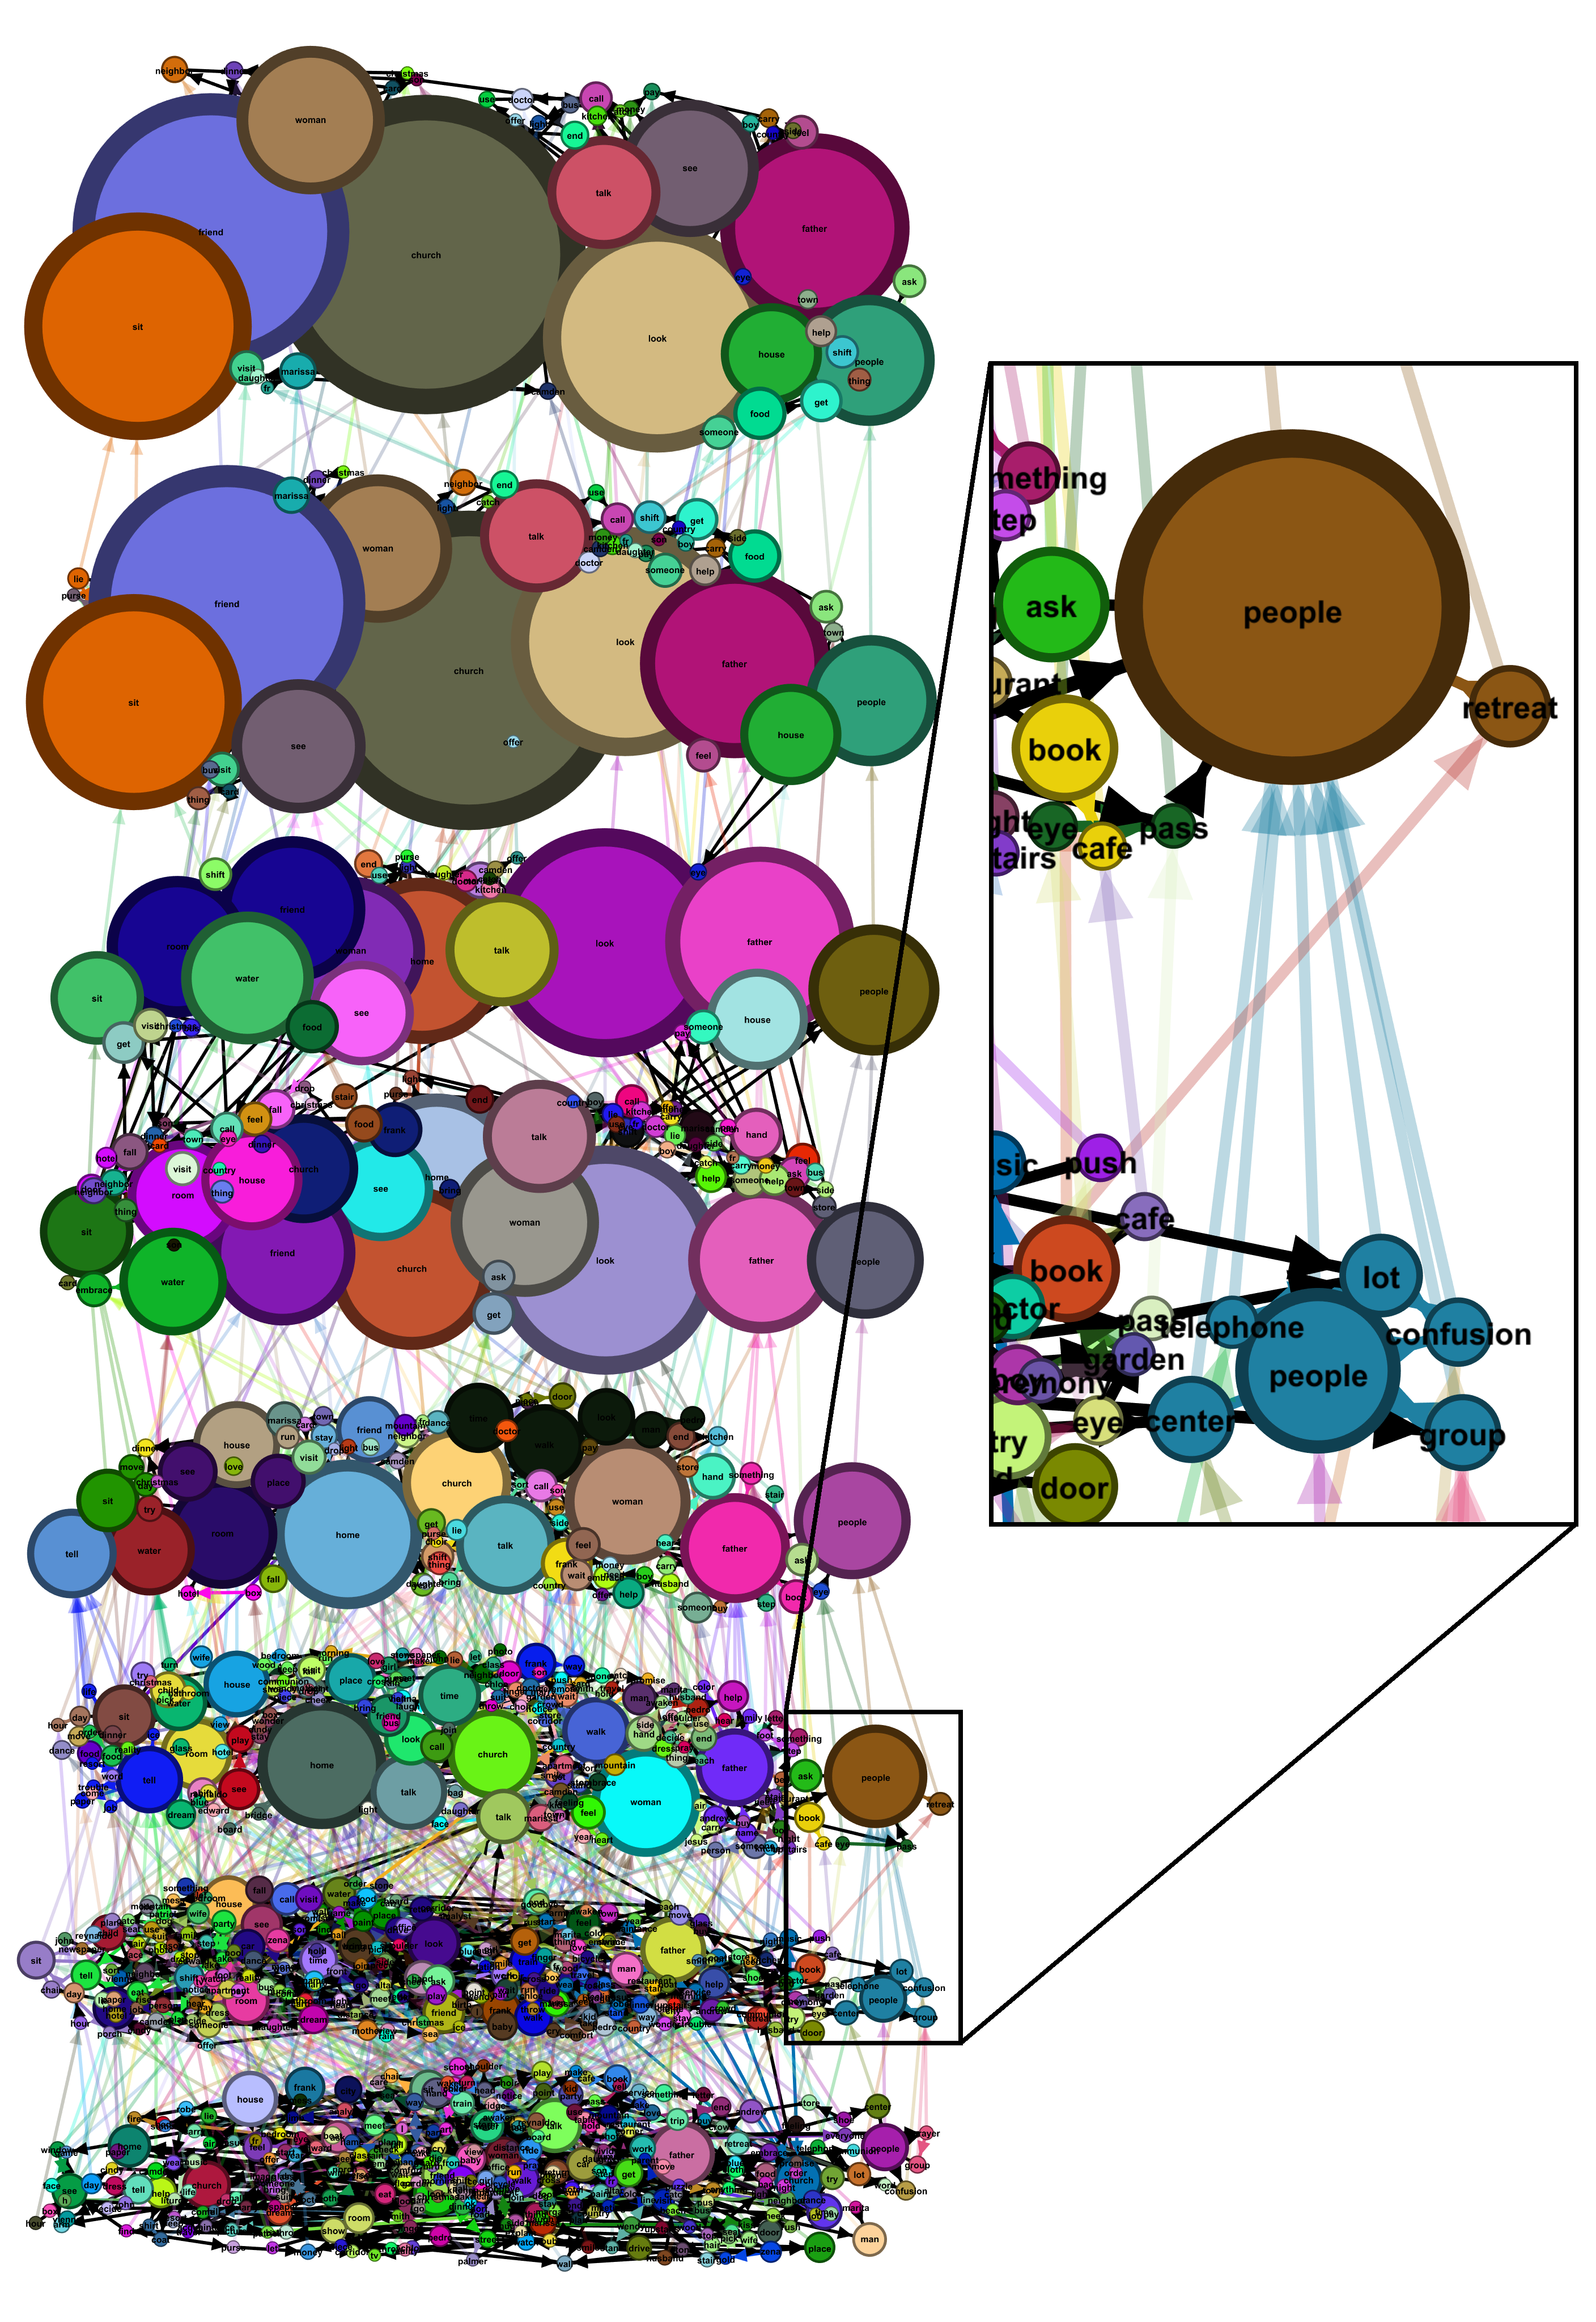
\includegraphics[width=1\textwidth]{Immagini/mlg_emma_focus_example}
    \caption{Grafo multi-livello del corpus di sogni di Emma}
    \label{fig:mlg-emma-example}
\end{figure}

Il rilevamento dei cicli, che identifica sequenze rilevanti di parole che riportano alla parola iniziale, potrebbero
rappresentare schemi influenti o temi ricorrenti nelle narrazioni dei sogni,
potenzialmente indicando collegamenti di pensiero persistenti nei sogni di Emma.
Si noti tuttavia che per l'elevato numero di sogni considerati e per la conseguente scelta del parametro di threshold,
la presenza di cicli è limitata a poche brevi sequenze di parole particolarmente correlate, date da gruppi di
parole come ``cake''-``party'', ``boat''-``lake''-``water'', ``trip''-``train''-``station'' oppure
``road''-``car''-``drive''-``hill''.
\'E interessante fare supposizioni su come queste sequenze possano fornire delle informazioni rilevanti proprio per
via del forte legame semantico che esse rappresentano.
Ad esempio la sequenza ``liturgy''-``church'-``music'' potrebbe indicare che per Emma il tema della musica è
fortemente associato al contesto della chiesa e alla liturgia, rispetto ad altri contesti che potrebbero
essere maggiormente attinenti per altre persone, come quello di un concerto o di un'accademia musicale.


L'individuazione delle componenti fortemente connesse al livello successivo potrebbe indicare unità tematiche coerenti
che, nel complesso delle narrazioni dei sogni, si co-occorrono e si interconnettono frequentemente tra loro rendendosi
mutualmente raggiungibili.
Queste componenti potrebbero rappresentare cluster di concetti o temi strettamente
interrelati che frequentemente co-occorrono e si interconnettono tra più sogni.
Come si può dedurre confrontando le dimensioni dei nodi al livello $2$ rispetto a quelle del livello precedente,
l'applicazione della contrazione per componenti fortemente connesse, in genere permette di individuare contesti
semanticamente più ampi di quelli visti per la contrazione per circuiti semplici.
Questo è dovuto da un lato alla natura delle componenti stesse, da un altro al fatto che la contrazione avviene
già ad un livello di astrazione superiore, in cui concetti strettamente collegati sono già stati raggruppati in unici
supernodi.
Esempi di insiemi di lemmi originali contenuti in componenti fortemente connesse individuate sono
``sit''-``chair''-``front''-``porch''-``seat''-``plane''
oppure ``lake''-``boat''-``water''-``rise''-``pool''-``swim''-``rush'', che racchiude uno dei circuiti semplici visti
in precedenza.

La contrazione per stelle, infine, permette di inglobare ulteriormente dei supernodi periferici ai quelli principali già
affermati nei primi livelli.
In questo modo lemmi e contesti che ``orbitano'' attorno ad altri e che, quindi,
ne siano strettamente dipendenti, vengono contratti in contesti più generali, espandendosi di una singola unità
di distanza di un arco ad ogni successivo livello.
Lo scopo di queste contrazioni altro non è che quello di far nascere dei macro-cluster che includano la maggior parte
delle parole originali, in maniera simile a come accade per alcuni strumenti di NLP, come i modelli di
\textit{word embedding}, le tecniche di \textit{topic modeling} e algoritmi di clustering semantico.
